\chapter{Introduction}
\label{introduction}
A Virtual Private Network (VPN) provides the illusion of a local area network
(LAN) spanning a wide area network (WAN) infrastructure by creating encrypted
and authenticated, secure\footnote{For the remainder of this proposal, unless
explicitly stated otherwise, security implies encryption and mutual
authentication between peers.} communication links amongst participants.
Common uses of VPNs include secure access to enterprise network resources from
remote/insecure locations, connecting distributed resources from multiple
sites, and establishing virtual LANs for multiplayer video games over the
Internet.  VPNs, in the context of this proposal, differ from others that
provide ```emulation of a private Wide Area Network (WAN) facility using IP
facilities' (including the public Internet or private IP backbones).
''~\cite{ip_vpns}.  These style of VPNs connect large sets of machines behind
routers to a virtual private WAN.

As a tool enabling collaborative environments, VPNs can be useful for many
different types of users.  If friends and family require computer assistance
and their computer guru no longer lives nearby, the guru can remotely log into
the machine using a VPN despite networking constraints between the two parties
so long as they both have Internet connections.  When traveling abroad, a user
may wish that their Internet traffic be kept private from the local network.  A 
VPN can be used to route all Internet packets through the user's home network,
ensuring the user's privacy.  Many computer and video games have multiplayer
networking components that require direct connectivity and games with
centralized servers bootstrapping multiplayer connectivity eventually lose
support.   Players of these games can continue playing with their remote friends
through VPNs.  Small and medium businesses may find VPNs useful for connecting
desktops and servers across distributed sites securing traffic to enterprise
networked resources.  Independent organizations that each have limited
resources can combine together their resources through a VPN to create a
powerful computing grid.

There are various VPN architectures that attempt to deal with the challenges
presented in these use cases.  In some cases one VPN approach may work,
where another is not applicable, and in some no current VPN approach is
applicable.  In general successful deployment and use of VPNs face the
following challenges:  
\begin{itemize}
\item \textbf{Configuration}:  Initial setup of the VPN.  Where will VPN
resources be located, what type of security credentials will be used, what are
the network parameters, how will users connect to the VPN.
\item \textbf{Peer Management}:  As peers and external resources desire to join
the system, security credentials need to be provided to both.  External
resources need to be linked to the rest of the system.  When peers misbehave,
their membership must be revoked.
\item \textbf{Connectivity}:  Peers may want to connect to a remote environment
or to each other.  Communicating through a central resource may create
bottlenecks, but doing so directly may be impossible due to restrictive network
environments.
\item \textbf{Privacy}:  When using a VPN, peers assume that their communication
is private.  VPNs that establish their links through a centralized system are
susceptible to man-in-the-middle attacks, though setting up decentralized
systems can be significantly more complicated.
\item \textbf{Permissions}:  Users must be administrators or given the ability
to run a VPN by an administrator, limiting their use in computing labs and
similar environments, where users are unable to run administrator privileged
software.
\end{itemize}

The key to using a VPN in collaborative environments is making it user-friendly
and scalable.  Applying these requisites to the challenges leads to the
following requirements:  a collaborative VPN should be easy to configure, such
that users should be able to deploy and use them without being experts in
operating systems (OSs) or networks; a single site to provide connectivity;;
adding new users and resources should be straight-forward using approaches
familiar to common users; peers should be able to connect to each other directly
if and when possible; not only should the communication in the system be secure
but so should the organization of the resources in the VPN; and users should be
able to connect to the VPN so long as there is Internet connectivity.  While
existing VPN are able to meet some of these requirements, they are unable to
meet them all.  Centralized approaches (e.g.  OpenVPN~\cite{openvpn}) by their
very nature require dedicated infrastructures and do not allow direct
communication between peers though when properly configured are able to able
to guarantee all-to-all communication regardless NAT and firewall conditions.
P2P-based approaches (e.g. Hamachi~\cite{hamachi}, Wippien~\cite{wippien},
Gbridge~\cite{gbridge}, PVC~\cite{pvc}) are vulnerable to man-in-the-middle
attacks if session management is handled by an external provider, rely on a
central resource for the creation of VPN links, and require managed relays if
direct peer communication across NATs and firewalls fails.  Decentralized
approaches require manual configuration of links between members of the virtual
network (e.g., ViNe~\cite{vine}, Violin~\cite{violin}, VNET~\cite{vnet},
tinc~\cite{tinc}).  Existing P2P approaches lack scalability (N2N~\cite{n2n}
and P2PVPN~\cite{p2pvpn}) or are difficult to configure and lack privacy
(I3~\cite{i3}).

This proposal focuses on VPNs useful for collaborative environments through
novel peer-to-peer (P2P) VPN systems.  In this proposal, I review the key
components of a VPN and either show how existing P2P systems can be used to
support the components or design and implement new features and systems as
necessary.  P2P systems align well with collaborative environments in large
part due to their decentralized and distributed nature; however, P2P presents
challenges in ensuring security and scalability.  While P2P systems can be used
to implement scalable autonomic and decentralized systems, when used in public
environments, they do not provide the security and isolation expected of a VPN
as they are easily compromised by malicious users.  Alternatively, the cost of
hosting a private overlay can out weigh the advantages in collaborative
environments.  My work extends from approaches that use P2P to implement
scalable virtual networks, IPOP~\cite{ipop} and I3~\cite{i3}, improving the work
of my predecessors by designing and implementing a system that provides privacy
or user-friendly configurability.  At the heart of my contribution are methods
enabling secure, user-friendly VPNs through the use of P2P systems.

\section{Virtual Private Network Basics}
VPNs consist of two components: clients that communicate with each other and
servers or overlays that provide the infrastructure for clients to find and
establish communication with each other.  From a user's perspective the
environment provided by a VPN client is the same regardless of how the server
or overlay is implemented.  The client's interface with the server can also
be abstracted such that clients are quite generic.

Figure~\ref{fig:vpn} abstracts the common features of all VPNs clients, a
service and a virtual network (VN) device providing communication with the VPN
system and host integration, respectively.  During initialization, the VPN
service authenticates with the system~\footnote{A system in this context refers
any portion of the VPN system including a central server, another VPN client,
or a relay.}, optionally, querying for information about the network, such as
network address space, address allocations, and domain name service (DNS)
servers.  At which point, the VPN enables secure communication amongst
participants.

Clients can authenticate with the overlay using a variety of methods.  A system
can be setup quickly by using no authentication or a shared secret such as a key
or a password.  Using accounts and passwords with or without a shared secret
provides individualized authentication, allowing an administrator to block all
users if the shared secret is compromised or individual users who act
maliciously.  In the most secure approaches, each client has a unique signed
certificate making brute force attacks very difficult.  The trade-offs in the
approaches come in terms of security, usability, and management.  While the use
of signed certificates provides better security than shared secrets,
certificates require more configuration and maintenance.  In a system comprising
of non-experts, like University VPNs, the usual setup uses a shared secret and
individual user accounts.  Secrets can be packaged with the VPN application, so
long as it is distributed through secure channels such as authenticated HTTPS.

A VN device allows applications to communicate transparently over the VPN.  The
VN device provides mechanisms for injecting incoming packets into and retrieving
outgoing packets from the networking stack, enabling the use of common network
APIs such as Berkeley Sockets, thereby allowing existing applications to work over
the VPN without modification.  While there are many different types of VN
devices, TAP~\cite{tap} stands out from the rest due to its open source and
pervasive nature.  TAP allows the creation of one or more Virtual Ethernet and
/ or IP devices and is available for almost all modern operating systems
including Windows, Linux, Mac OS/X, BSD, and Solaris.  A TAP device presents
itself as a character device providing read and write operations.  Incoming
packets from the VPN are written to the TAP device and the networking stack in
the OS delivers the packet to the appropriate socket.  Outgoing packets from
local sockets are read from the TAP device.

VN devices can be configured manually through command-line tools or OS' APIs or
dynamically by the universally supported dynamic host configuration process
(DHCP)~\cite{dhcp0, dhcp1}.  Upon the VN device obtaining an IP address, the
system adds a new rule to the routing table that directs all packets sent to
the VPN address space to be directed to the VN device.  Packets read from the
TAP device are encrypted and sent to the overlay via the VPN client.  The
overlay delivers the packet to another client or a server with a VN stack
enabled.  Received packets are decrypted, verified for authenticity, and then
written to the VN device.  In most cases, the IP layer header remains unchanged,
while VPN configuration determines how the Ethernet header is handled.

\section{Computer Network Architectures}
All models for computer communication in distributed systems fall under two
categories:  centralized and decentralized.  They can be further divided into
hybrid systems with centralized session management and decentralized
communication and self-configuring, dynamics P2P systems.  The architectures
commonly used for implementing VPN systems are:

\begin{itemize}
\item \textbf{Centralized Organization and Communication} - These are client
server systems, where all distributed peers both locally and remote are clients
discovering and connecting, or organizing, through a dedicated centralized
resource. Clients never communicate with each other directly only, but rather
every message between two clients must traverse the server.  For instance, most
online social networks (OSNs) are representative of these type of systems.
Users of OSNs like Facebook~\cite{facebook} and MySpace~\cite{myspace}
communicate through centralized environments never directly to each other's
computers.  OpenVPN~\cite{openvpn} represents this domain in VPNs.  These
systems rely on on dedicated resources.  In the situation that a server goes
offline or becomes overwhelmed by the clients, the system is rendered useless.
\item \textbf{Centralized Organization and Decentralized Communication} - The
first set of popular P2P systems, such as the original Napster, Kazaa, and VPNs
like Hamachi~\cite{hamachi}, fall into this category.  Similar to the
client-server model, clients connect to a server to find other clients, though
instead of communicating through the server, the clients form direct
connections with each other.  These approaches are limited by network address
translation (NAT) and firewalls that may prevent peers from communicating with
each other.  In these cases, the central server may act as a relay allowing the
two clients to communicate through it.  Unlike systems using centralized
communication, these systems are less susceptible to being overwhelmed by
client traffic and even if the server goes offline existing client links remain
active, though new connections cannot be formed.
\item \textbf{Decentralized with Manual Organization} - To address the issues
of a central system going offline, many distributed servers may be used and
clients can be configured to connect to any number of them creating an overlay.
In these systems, servers are explicitly configured to communicate with other
remote and local servers.  Though this approach improves upon the issues
inherent with completely centralized architectures, if a site goes offline any
systems communicating through it will no longer be connected to the rest of the
system until the administrator creates additional links or the site becomes
active again.  Clients in these systems do not typically form direct links with
each other, rather they route packets through the overlay.  This approach has
been used to create scalable VPNs, like ViNe~\cite{vine}, VNET~\cite{vnet},
Violin~\cite{violin}, and Layer 2 Tunneling Protocol based VPNs~\cite{l2tp}.
\item \textbf{Decentralized with Automatic Organization} - The last model falls
under systems that self-organize.  In this environment, there is no distinction
amongst peers as they act as both client and servers, i.e., a P2P system or
overlay.  P2P systems are usually distributed with a list of common peers.  When
attempting to connect with the P2P overlay, a peer randomly selects peers on
this list until it is able to connect with one.  This connection is then used
to form connections with other peers currently in the overlay.  The overlay
can be organized in two different forms: randomly or deterministically
creating unstructured or structured overlays, respectively.  In an unstructured
overlay, links are formed arbitrarily, thus a peer searches for another peer
by broadcasting the message or using stochastic techniques.  In structured
overlays, peers organize into topologies by deterministically forming
connections with peers nearby in the overlay address space creating ring and
hybercubes.  Peers can be found deterministically using greedy routing
approaches in usually $O(\log(N))$ time.  Gnutella~\cite{gnutella} file sharing
system and Skype~\cite{skype} are popular examples of unstructured systems,
while P2PSIP~\cite{p2psip} and distributed hash tables (DHTs)~\cite{chord} are
popular in structured systems.  The challenges to unstructured systems is
finding data objects in reasonable amount of time, while structured systems
suffer when large amount of peers join or leave the system, known as
churn~\cite{opendht}.  In general, both approaches are difficult to secure due
to their typical application.  When used in private environments though, they
have been shown to be very useful, exemplified by Dynamo~\cite{dynamo} or
BigTable~\cite{bigtable}.
\end{itemize}

This proposal uses structured overlays as the foundation in building scalable,
decentralized VPNs, Chapter~\ref{structured_p2p} provides a more detailed
review of structured overlays and challenges in decentralized communication
with emphasis on security, establishing connections, and reliability.  I also
provide solution to these challenges in the form of private virtual overlays
bootstrapping secure overlays using public free-to-join overlays, a
decentralized relay system when direct NAT or firewall traversal fails, and an
overlay-aware TCP enabling reliable and efficient communication over unreliable
links.

\section{Contributions}
Applying the challenges listed in the introduction to collaborative
environments the resulting requirements are self-configuring environments
enabling even non-experts to setup, deploy, and manage their own VPNs; peers
should communicate with each other directly when possible or through efficient
indirect paths when constrained; the system should be reliable and ensure the
privacy of its users; and users should be able to access the VPN regardless of
their user privileges so long as they can run network applications.  To address
these requirements, I propose a novel GroupVPN using structured overlays
consisting of the following novel contributions:

\begin{itemize}
\item \textbf{Self-Configuring VPN Architectures}: Many existing VPN approaches
require the users to setup their environment and do not provide a plug and play
system.  In addition, different environments call for different types of VPNs,
explicitly, individual users connect via their own VPN connections, while
clusters may benefit from a shared VPN or may desire fault tolerance of having
many but do not want the communication overhead when talking to VPN peers on
the LAN.  I address this issue with a self-configuring VPN approach that can be
applied to various local environments scaling from a single computer to many.
\item \textbf{Virtual Private Overlays}:  At any given time, peers may or may
not be connected to the overlay.  When used in small groups, most or all
members may be behind NATs or remain online for short periods of time.  Creating
a situation, where not a single user on a publicly addressable resource will be
online, limiting the use of private overlays.  To address this issue, I propose
the use of a public free-to-join overlay to bootstrap into a private overlay.
Peers use the public overlay to find each other and exchange connection
information using secure messages.  Only peers with appropriate security
credentials are able to join the private overlay.
\item \textbf{Userspace Virtual Networking Stack}: To address the case where
users do not have permissions to run VPNs, I plan on designing and implementing
a limited permissions VPN proxy system allowing connection to regular VPNs.
\item \textbf{Overlay Communication Models}: In my experience, when using the
overlay based connections, performance suffers due to being processed by the
overlay's state machine.  I will work towards addressing this issue by
investigating different models for using overlays to establish direct
communication:  communicating through the overlays state machine, bypassing the
overlay's state machine but reusing its connection management, and creating
links separate from the overlay.
\item \textbf{Overlay-Aware TCP}: Overlays consist of peers connecting and
disconnecting at random typically connectioning through UDP to reduce resource
load and provide efficient NAT and firewall traversal capabilities.  Therefore,
large streams of data cannot be sent reliably through the overlay.  This is not
an issue when a VPN has administrator permission enabling the reuse of the OS'
network stack including TCP.  For situations that lack this ability, I will
design a TCP stack with focus on efficient and reliable streaming using
overlays.
\item \textbf{Decentralized Relays}:  In collaborative environments, most peers
are behind NATs and potentially firewalls as well.  While in general most
NATs are traversable through existing approaches, not all are.  Firewalls only
complicate the matter.  While these peers may be able to communicate through
the overlay, as the overlay grows, this latency can become a hindrace to
usability and interactivity.  To improve this situation, I propose the creation
of autonomic 2-hop relays between the peers.
\item \textbf{P2P VPN Enabled Internet Traffic Tunneling}: When in insecure
environments such as browsing private information in a coffee shop, users may
desire to prevent local users and administrators from sniffing their traffic.
Traditional VPNs support this behavior, but the approach is difficult to
implement in P2P systems due to their dynamic nature.  Currently, no
decentralized VPN supports the ability to perform this behavior.  I propose a
method that not only works for decentralized and P2P systems but ensures a
greater level of security than existing approaches by securing other non-VPN
communication between the peer and gateway resources.
\end{itemize}

In order to assess the practical applicability of  the propose work and to
quantitatively evaluate its performance in relaistic wide-area environments,
this thesis has a significant component in the design, deployment, and
evaluation of functional systems that implement the proposed approaches with
emphasis in the realms of online social networking and grid computing.  I will
determine feasibility of implementing an online social network using the 
structured overlays with particular focus on the use of private virtual
overlays as social network profiles or profile overlays.  In addition, the
primary motivation for my work has been the use of self-configuring VPNs and
systems for grid computing.  In this proposal, my culminating work, I will
describe how this system can be used to create a novel self-configuring grid
system that allows users who have limited knowledge of operating systems,
networks, and computers to create their own grids in a matter of minutes.

The rest of this proposal is organized as follows.  In
Chapter~\ref{structured_p2p}, I present an in depth analysis of structured
overlays including a review of NAT constraints and traversal and then explore
the use of decentralized relays.  This leads into Chapter~\ref{vpo}, which
discusses security issues in structured overlays and a solution enabling users
to create their own private pools using public overlays.  Chapter~\ref{vpns}
continues the discussion of VPNs with focus on the different architectures 
focusing on both local and network configuration.  Chapters \ref{gridappliance}
and \ref{spo} present two distinct applications of the novel overlay and VPN
approaches pursued in this proposal.  Finally, I conclude the proposal by 
discussing real systems and future work in Chapter~\ref{conclusion}.

\section{Figures and Tables}
\begin{figure}[ht]
\centering
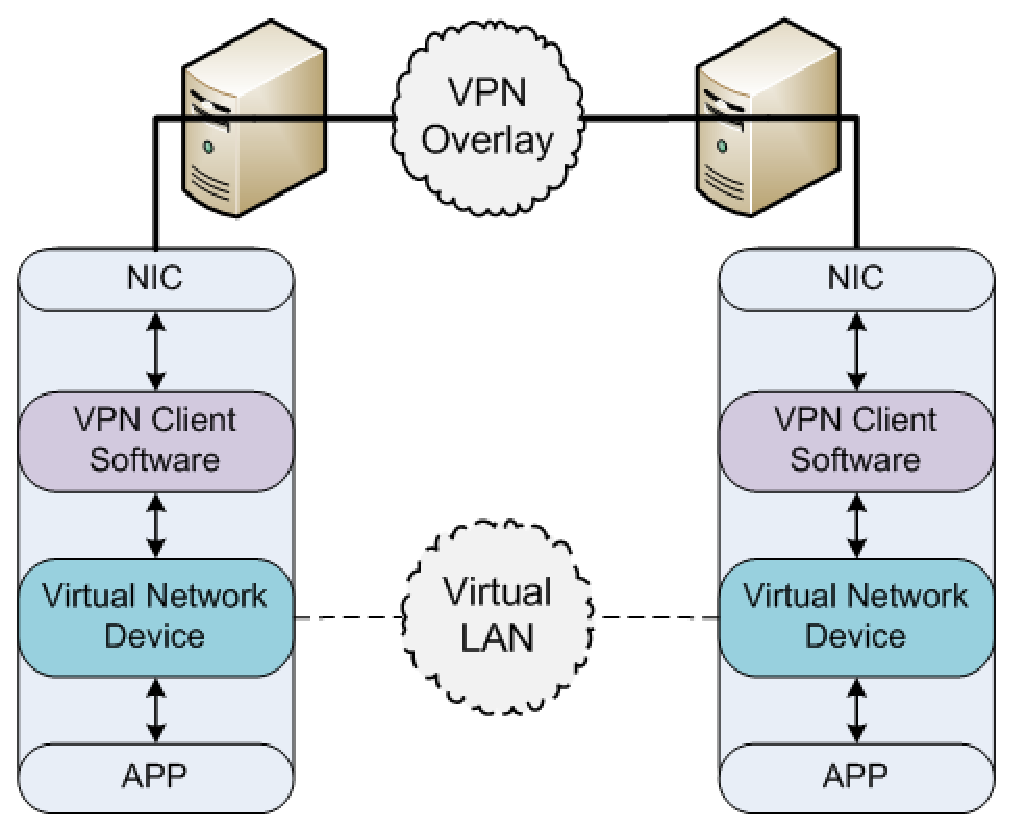
\epsfig{file=figs/vpn.png.eps, width=4in}
\caption[A typical VPN client]{A typical VPN client.  A VN device makes
application interaction with the VPN transparent.  Packets going to the VPN
destination are sent by routing rules to the VN device interfaced by the VPN
client.  The VPN client sends and receives packets from other VPN participants
via the hosts physical network device.}
\label{fig:vpn}
\end{figure}
